% !TeX spellcheck = en-US
% !TeX encoding = utf8
% !TeX program = pdflatex
% !BIB program = biber
% -*- coding:utf-8 mod:LaTeX -*-


% vv  scroll down to line 200 for content  vv


\let\ifdeutsch\iffalse
\let\ifenglish\iftrue


\input{pre-documentclass}
\documentclass[
  %
  %ngerman, %%% Add if you write in German.
  %
  % fontsize=11pt is the standard
  a4paper,  % Standard format - only KOMAScript uses paper=a4 - https://tex.stackexchange.com/a/61044/9075
  twoside,  % we are optimizing for both screen and two-side printing. So the page numbers will jump, but the content is configured to stay in the middle (by using the geometry package)
  bibliography=totoc,
  %               idxtotoc,   %Index ins Inhaltsverzeichnis
  %               liststotoc, %List of X ins Inhaltsverzeichnis, mit liststotocnumbered werden die Abbildungsverzeichnisse nummeriert
  headsepline,
  cleardoublepage=empty,
  parskip=half,
  %               draft    % um zu sehen, wo noch nachgebessert werden muss - wichtig, da Bindungskorrektur mit drin
  draft=false
]{scrbook}
\input{config}


\usepackage[
  title={Alerting Users to Phishing Threats: A Comprehensive Evaluation of Warning Techniques}, % Do not forget to capitalize your title correctly, you may use the following page to help you: https://capitalizemytitle.com/
  author={Yunus Emre Yavuz},
  orcid=0009-0009-6762-8269, % get your own ORCID via https://orcid.org/
  email={yunus.yavuz@campus.lmu.de},
  type=bachelor,
  institute={Institut für Informatik}, % or other institute names - or just a plain string using {Demo\\Demo...}
  examiner={Univ.-Prof.\ Dr.\ Florian Alt},
  supervisor={Dr.\ Verena Distler,\\Felix Dietz,\ M.Sc.},
  startdate={January 20, 2024},
  enddate={soon},
  % Falls keine Lizenz gewünscht wird bitte auf "none" setzen
  % Die Lizenz erlaubt es zu nichtkommerziellen Zwecken die Arbeit zu
  % vervielfältigen und Kopien zu machen. Dabei muss aber immer der Autor
  % angegeben werden. Eine kommerzielle Verwertung ist für den Autor
  % weiter möglich.
  copyright=ccbysa, % ccbysa, ccbynosa, cc0, none
  language=english
]{lmu-thesis-cover}

\usepackage{tabularx}
\usepackage{caption}
\usepackage{subcaption}
\usepackage{tikz-uml}
\usepackage{float}
\usepackage{pgfplots}
\usepgfplotslibrary{statistics}
\pgfplotsset{width=10cm,compat=1.15}
% Hier stehen alle Abkürzungen
\newacronym{aoi}{AOI}{Area of Interest}
\newacronym{qda}{QDA}{Qualitative Data Analysis}
\newacronym{ati-s}{ATI-S}{Affinity for Technology Interaction Short Scale}


\makeindex


\begin{document}

%tex4ht-Konvertierung verschönern
\iftex4ht
  % tell tex4ht to create picures also for formulas starting with '$'
  % WARNING: a tex4ht run now takes forever!
  \Configure{$}{\PicMath}{\EndPicMath}{}
  %$ % <- syntax highlighting fix for emacs
  \Css{body {text-align:justify;}}

  %conversion of .pdf to .png
  \Configure{graphics*}
  {pdf}
  {\Needs{"convert \csname Gin@base\endcsname.pdf
      \csname Gin@base\endcsname.png"}%
    \Picture[pict]{\csname Gin@base\endcsname.png}%
  }
\fi

%\VerbatimFootnotes %verbatim text in Fußnoten erlauben. Geht normalerweise nicht.

\input{commands}
\pagenumbering{arabic}
\Coverpage
\Copyright
%Eigener Seitenstil fuer die Kurzfassung und das Inhaltsverzeichnis
\deftriplepagestyle{preamble}{}{}{}{}{}{\pagemark}
%Doku zu deftriplepagestyle: scrguide.pdf
\pagestyle{preamble}
\renewcommand*{\chapterpagestyle}{preamble}



%Kurzfassung / abstract
%auch im Stil vom Inhaltsverzeichnis
\section*{Kurzfassung}
Phishing-Angriffe sind trotz diverser Fortschritte im Bereich der Cybersicherheit nach wie vor eine große Bedrohung. Diese Arbeit befasst sich mit der Verbesserung der Erkennung von und Reaktion auf Phishing durch die Gestaltung und Implementierung visueller Warnungen in E-Mail-Clients. Über einen Zeitraum von zwei Wochen wurde eine Mixed-Methods-Studie mit 16 Teilnehmern durchgeführt, in der Eye-Tracking-Technologie und qualitatives Feedback integriert wurden, um die Interaktionen mit verschiedenen Phishing-Warnungen in Mozilla Thunderbird zu bewerten. \newline
Die Studie ergab, dass Warnungen, die direkt in den E-Mail-Inhalt integriert sind, das Engagement der Benutzer und die Reaktionszeiten im Vergleich zu peripheren Warnungen deutlich verbessern. Eye-Tracking-Daten zeigten, dass unmittelbare und prominent platzierte Warnungen effektiver sind, während periphere Warnungen tendenziell erst später wahrgenommen werden, was ihre Effektivität in realen Szenarien verringern könnte. Qualitatives Feedback unterstrich die Bedeutung von Klarheit, Kontext und lehrreichen Inhalten in den Warnhinweisen, um das Verständnis der Benutzer zu verbessern und Phishing-Angriffe zu verhindern. \newline
Diese Ergebnisse legen nahe, dass die Gestaltung von Phishing-Warnungen erhebliche Auswirkungen auf die Cybersicherheit haben kann. Durch die Konzentration auf benutzerzentrierte Warnhinweise, die sowohl auffällig als auch informativ sind, können die Abwehrmechanismen von Phishing-Angriffen erheblich gestärkt werden. Diese Forschungsarbeit leistet einen Beitrag zum breiteren Feld der Cybersicherheit, indem sie evidenzbasierte Empfehlungen für die Gestaltung effektiver Phishing-Warnungen liefert, die darauf abzielen, die Prävalenz und die Auswirkungen von Phishing zu reduzieren. 

%\todo{Short summary of the thesis. Here, the following questions should be answered:}
%\todo{What is the specific problem addressed?}
%\todo{What have you done?}
%\todo{What did you find out?}
%\todo{What are the implications on a larger scale?}
%\todo{Should be around 0.5 pages. Not longer than 1 page.}

\cleardoublepage

\section*{Abstract} 
Phishing attacks remain a significant threat despite advancements in cybersecurity. This thesis addresses the enhancing of user detection and response to phishing through the design and implementation of visual warnings within email clients. Over a two-week period, a mixed-methods study involving 16 participants was conducted, integrating eye-tracking technology and qualitative feedback to assess interactions with various phishing warning designs in Mozilla Thunderbird. \newline
The study found that warnings directly integrated within the email content significantly improve user engagement and response times compared to peripheral warnings. Eye-tracking data revealed that immediate and prominently placed warnings are more effective, while peripheral warnings tend to be noticed later, potentially reducing their effectiveness in real-world scenarios. Qualitative feedback highlighted the importance of clarity, context, and educational content in warnings to enhance user understanding and prevent phishing attacks. \newline
These findings suggest that the design of phishing warnings can have substantial implications for cybersecurity. By focusing on user-centric warning designs that are both noticeable and informative, phishing defense mechanisms can be significantly strengthened. This research contributes to the broader cybersecurity field by providing evidence-based recommendations for designing effective phishing warnings, aiming to reduce the prevalence and impact of phishing attacks across digital platforms.



%\todo{Short summary of the thesis. Here, the following questions should be answered:}
%\todo{What is the specific problem addressed?}
%\todo{What have you done?}
%\todo{What did you find out?}
%\todo{What are the implications on a larger scale?}
%\todo{Should be around 0.5 pages. Not longer than 1 page.}

\cleardoublepage


% BEGIN: Verzeichnisse

\iftex4ht
\else
  \microtypesetup{protrusion=false}
\fi

%%%
% Literaturverzeichnis ins TOC mit aufnehmen, aber nur wenn nichts anderes mehr hilft!
% \addcontentsline{toc}{chapter}{Literaturverzeichnis}
%
% oder zB
%\addcontentsline{toc}{section}{Abkürzungsverzeichnis}
%
%%%

%Produce table of contents
%
%In case you have trouble with headings reaching into the page numbers, enable the following three lines.
%Hint by http://golatex.de/inhaltsverzeichnis-schreibt-ueber-rand-t3106.html
%
%\makeatletter
%\renewcommand{\@pnumwidth}{2em}
%\makeatother
%
\tableofcontents

% Bei einem ungünstigen Seitenumbruch im Inhaltsverzeichnis, kann dieser mit
% \addtocontents{toc}{\protect\newpage}
% an der passenden Stelle im Fließtext erzwungen werden.

\listoffigures
\listoftables


% Control List of Listings
\let\iflistings\iffalse
%Wird nur bei Verwendung von der lstlisting-Umgebung mit dem "caption"-Parameter benoetigt
%\lstlistoflistings
%ansonsten:
\iflistings
  \ifdeutsch
    \listof{Listing}{Verzeichnis der Listings}
  \else
    \listof{Listing}{List of Listings}
  \fi
\fi

% Control List of Algorithms
\let\ifalgorithms\iffalse
\ifalgorithms
  %mittels \newfloat wurde die Algorithmus-Gleitumgebung definiert.
  %Mit folgendem Befehl werden alle floats dieses Typs ausgegeben
  \ifdeutsch
    \listof{Algorithmus}{Verzeichnis der Algorithmen}
  \else
    \listof{Algorithmus}{List of Algorithms}
  \fi
  %\listofalgorithms %Ist nur für Algorithmen, die mittels \begin{algorithm} umschlossen werden, nötig
\fi

% Control Glossary
%\let\ifglossary\iffalse
%\ifglossary
  %\printnoidxglossaries
%\fi

\iftex4ht
\else
  %Optischen Randausgleich und Grauwertkorrektur wieder aktivieren
  \microtypesetup{protrusion=true}
\fi

% END: Verzeichnisse


% Headline and footline
\renewcommand*{\chapterpagestyle}{scrplain}
\pagestyle{scrheadings}
\pagestyle{scrheadings}
\ihead[]{}
\chead[]{}
\ohead[]{\headmark}
\cfoot[]{}
\ofoot[\usekomafont{pagenumber}\thepage]{\usekomafont{pagenumber}\thepage}
\ifoot[]{}


%% vv  scroll down for content  vv %%































%%%%%%%%%%%%%%%%%%%%%%%%%%%%%%%%%%%%%%%%%%%%%%%%%%%%%%%%%%%%%%%%%%%%%%%%%%%%%%
%
% Main content starts here
%
%%%%%%%%%%%%%%%%%%%%%%%%%%%%%%%%%%%%%%%%%%%%%%%%%%%%%%%%%%%%%%%%%%%%%%%%%%%%%%


\chapter{Introduction}
\label{sec:introduction}
% First Paragraph
% CORE MESSAGE OF THIS PARAGRAPH:
%\todo{P1.1. What is the large scope of the problem?}
%\todo{P1.2. What is the specific problem?}
In today's digital age, the internet is integral to daily activities such as communication, transactions, and accessing information. Yet, this increased dependency brings heightened security risks, especially from phishing attacks. Phishing, a prevalent cyber threat, involves deceiving individuals into revealing sensitive information by masquerading as a trustworthy entity in digital communications. There is a vast amount of phishing vectors, such as SMS, social media or email, with the latter being the most common medium for phishing attacks \cite{verizon}. These attacks are used to direct victims to fraudulent websites where they are coerced into providing personal and financial details, allowing attackers unauthorized access to accounts \cite{Wang2012}. \newline 
The impact of phishing extends beyond individual victims to organizations worldwide, causing significant financial losses and eroding trust in digital systems. In the second quarter of 2023 alone, the Anti-Phishing Working Group (AWPG) observed 1,286,208 phishing attacks \cite{apwg}. Despite the deployment of various anti-phishing technologies, the human factor remains a critical vulnerability. The effectiveness of phishing warnings, therefore, is paramount in the cybersecurity defense arsenal. These warnings, if designed and implemented effectively, can play a crucial role in educating users and averting the success of phishing attacks. \par
% Second Paragraph
% CORE MESSAGE OF THIS PARAGRAPH:
%\todo{P2.1. The second paragraph should be about what have others been doing}
%\todo{P2.2. Why is the problem important? Why was this work carried out?}
In response to the escalating threat of phishing attacks, numerous efforts have been undertaken by cybersecurity experts and organizations to mitigate the risks. These include the development of algorithms for threat detection \cite{thakur} and the implementation of user awareness programs \cite{jampen}. Users' ability to detect and respond to phishing attempts is critical, prompting a shift toward developing more user-centered security solutions. These solutions emphasize visual warnings that act as direct interventions, alerting users to potential threats. However, the effectiveness of such warnings hinges on several factors that this study aims to explore and understand. \par
% Third Paragraph
% CORE MESSAGE OF THIS PARAGRAPH:
%\todo{P3.1. What have you done?}
%\todo{P3.2. What is new about your work?}
For our study, we developed mock-up visual warnings to simulate real alerts in an email client and expanded their functionality with a custom plugin for Mozilla Thunderbird, a widely-used open-source email client chosen for its adaptability. This plugin enhances the visual presentation of phishing warnings, utilizing common design principles to capture users' attention more effectively. \newline
We created a unique set of emails incorporating both regular communications and mock phishing scenarios to simulate a realistic email environment, providing a robust platform for our user study. Using eye-tracking technology and detailed user feedback, we explored how users perceive, understand, and react to various visual warning strategies. This investigation offers insights into the design of more effective phishing warnings and highlights the importance of user interface design in cybersecurity. By focusing on user-centric design elements, our study aims to improve how visual cues are used to strengthen defenses against phishing attacks. Our research is structured around the following research questions:

\begin{itemize}
    \item RQ1: How do users' perceptions differ in response to various phishing warnings in email interfaces, and which type is perceived as the most effective? \textit{Here, "effective" refers to the ability of the warnings to increase user awareness, prompt appropriate user actions to mitigate risk (e.g., not clicking on malicious links), and enhance recognition of phishing threats in future encounters.}
        \begin{itemize}
            \item How do users perceive the helpfulness of each warning type?
        \end{itemize}
        \begin{itemize}
            \item Which warning design do users prefer and why?
        \end{itemize}
    \item RQ2: What common gaze patterns emerge among users when scanning email content, and how can these patterns help with the strategic placement of phishing warnings to maximize user attention?
\end{itemize}

To adress these research question we have laid out the following objectives for our study:

\begin{enumerate}
    \item \textit{Evaluating Visual Warning Strategies:} We aim to examine the effectiveness of various visual elements (banner placement, animations) in warning designs in terms of their immediate recognizability and understandability.
    \item \textit{Analyzing Attention Distribution:} Using eye-tracking technology, we plan to identify which visual elements attract users' attention and how these elements influence perception and behaviour.
    \item \textit{Assessing User Reactions:} Through interviews with participants, we intend to capture their subjective evaluations and opinions regarding the different warning types. This includes exploring user trust and their perception on the warnings helpfulness.
    \item \textit{Establishing Best Practices:} Based on the collected data and user feedback, we seek to identify design principles that maximize the effectiveness of phishing warnings.
\end{enumerate}

% Fourth paragraph
% CORE MESSAGE OF THIS PARAGRAPH:
%\todo{P4.1. What did you find out? What are the concrete results?}
%\todo{P4.2. What are the implications? What does this mean for the bigger picture?}
In summary, our research reveals that effectively designed phishing warnings can significantly influence users' abilities to recognize and respond to phishing attempts. Eye-tracking data confirmed that warnings integrated within the email body are noticed and acted upon more swiftly than those placed peripherally or appearing with a delay. Qualitative feedback underscored the importance of clear, contextual information within these warnings, enhancing users' understanding of potential threats. \newline
The implications of these results are substantial, advocating for a shift in how cybersecurity defenses are structured. As phishing tactics evolve, the need for warnings that seamlessly integrate into users' workflows and effectively communicate risks becomes increasingly critical. By focusing on the development of user friendly and informative warning systems, we can better equip individuals to combat phishing threats, potentially reducing the success rate of such attacks across various platforms. 

%LaTeX hints are provided in \autoref{chap:latexhints}.

\chapter{Background and Related Work}
\label{sec:relatedwork}

Phishing attacks represent a significant and ever-evolving challenge in the realm of cybersecurity. This section provides an overview of key research areas that are crucial in understanding and combating these threats.  From the psychology underpinning social engineering tactics to the necessity of effective phishing training for users and the latest in phishing detection technologies, each area offers vital insights.

\section{Previous Approaches to Combating Phishing}
\textbf{Technical Detection Strategies}

Phishing detection technologies are essential tools, designed to identify and mitigate phishing attempts across various digital platforms. Among these technologies, email client spam filters, with phishing emails being a subset of spam mails, represent a fundamental line of defense, filtering out potential phishing emails based on specific criteria such as sender reputation \cite{shi} or message content \cite{alexy}.

In their paper, Bhomwick et al. \cite{alexy} delve into the evolution of machine learning techniques in the realm of email spam filtering. They chart the journey from initial heuristic-based approaches to the adoption of sophisticated machine learning models, capable of dynamically adapting to the continually evolving strategies employed by spammers. The paper not only highlights the effectiveness of these techniques but also points towards future directions for research in improving spam detection mechanisms.

Another approach in phishing detection is explored by Md. Abu Ashraf Siddiq et al. \cite{siddiq}, utilizing deep learning techniques. Their study, employing neural networks, showcases the potential of deep learning in accurately identifying phishing websites, with achievements of up to 94.8\% accuracy. This highlights deep learning's pivotal role in cybersecurity, especially in distinguishing malicious sites, and emphasizes its contribution to advancing phishing detection systems.

\textbf{User Education and Training}

Understanding the mechanisms behind phishing attacks and the reasons users fall prey to them is essential in developing effective countermeasures. A key vulnerability is the general lack of cybersecurity awareness among users, rendering them susceptible to manipulation by attackers. In their paper Dhamija et al. \cite{dhamija} this issue is highlighted, pointing out the critical need for enhanced user understanding to mitigate vulnerability to phishing shemes. 

To adress this gap, various training methods have been explored, aiming to improve user ability to recognize and resist phishing attempts. Research by Sheng et al. \cite{sheng} showcases an innovative approach in phishing education through the 'Anti-Phishing Phil' game. This research demonstrates that integrating educational content with interactive gameplay can significantly increase the efficacy of cybersecurity training. Such engaging methods not only educate but also actively involve users in the learning process, making the lessons more memorable and practical. 

Further emphasizing the importance of user education, Kumaguru et al. \cite{kumaraguru} investigated the impact of training on users' abilites to distinguish between legitimate and fraudulent websites. Their findings underscore the effectiveness of well-crafted educational programs in empowering users to safeguard themselves against phishing threats. 

Additionally, Wash's article \cite{wash} on how IT experts detect phishing emails provides a unique perspective on the cognitive strategies employed by experienced professionals. By interviewing IT experts, Wash explains a three-stage process these professionals use: sensemaking, suspicion, and decision-making, when evaluating the legitimacy of an email. This approach underscores the depth of expertise and vigilance required to effectively identify phishing attempts, highlighting the potential benefits of training programs that enhance these cognitive skills among general users.

In conclusion, the success of phishing attacks largely hinges on exploiting user vulnerabilities, primarily due to inadequate cybersecurity awareness. The research reviewed here underscores the significance of user education in fortifying defenses against such threats.

\section{Phishing Techniques}
Phishing attacks utilize a blend of technical and psychological tactics to extract sensitive information from victims, as detailed by Alkhalil et al. \cite{alkhalil}. These attacks involve various stages, from target research to the deployment of deceptive messages designed to look trustworthy.

Alkhalil et al. identify several prevalent phishing techniques:
\begin{itemize}
    \item \textit{Email Phishing:} The primary method where attackers send fraudulent emails mimicking legitimate sources to steal personal information.
    \item \textit{Spear Phishing and Whaling:} Highly targeted forms that use personalized information to increase the attack's credibility.
    \item \textit{Vishing (Voice Phishing) and SMiShing (SMS Phishing):} Phishing via phone calls and SMS that exploit the user's trust in mobile communications.
    \item \textit{Website Forgery:} Creating counterfeit websites that replicate genuine ones to capture personal data.
    \item \textit{Social Media Phishing:} Using social platforms to trick users into revealing sensitive data through deceptive posts or messages.
\end{itemize}


\section{Social Engineering and the Human Factor}
Social engineering is described as an attack type where the assailant exploits human vulnerabilities through social interaction to compromise cybersecurity goals like confidentiality, integrity, and availability of cyber elements. Unlike traditional attacks that may require overcoming technical barriers, social engineering attacks manipulate human psychology to bypass security measures. It's particularly challenging to defend against because it preys on innate human traits, which can often be turned into security vulnerabilities by skilled attackers \cite{Wang2021}.

The study by Albladi et al. \cite{albladi} examines factors that predict individuals' vulnerability to social engineering in social networks. It proposes a model incorporating user characteristics such as level of involvement, social network experience, and perceptual factors like risk perception and competence. This research aims to identify the most vulnerable users for targeted training programs, contributing to safer social networking practices.

The study by Koddebusch \cite{koddebusch} highlights the specific persuasive techniques employed in phishing emails, such as invoking authority or urgency, which effectively manipulate users' decision-making processes. This manipulation illustrates how cyber attackers exploit psychological triggers to induce actions that users might otherwise consider risky or unnecessary. Koddebusch's findings provide empirical evidence that these persuasion strategies significantly increase the success rate of phishing attacks, underscoring the critical need for awareness and training that can help individuals recognize and resist such tactics.

The paper by Abdrabou et al. \cite{abdrabou} investigates how phishing emails affect user behavior by tracking their gaze and mouse movements during an email sorting task. The study aims to understand if these physiological and behavioral cues can serve as indicators of exposure to phishing attacks, which are often designed to manipulate users into revealing sensitive information. Their findings suggest that subtle changes in behavior, such as eye movements or mouse dynamics, could potentially be used to identify when users are interacting with phishing content. 

Distler's study \cite{distler} examines the impact of various contextual factors on individuals' responses to phishing within an organizational setting. Using an in-situ deception methodology with 14 participants in their real work environments, the study reveals that contexts significantly influence the likelihood of falling for phishing emails. Distler's findings underscore the importance of contextualized training and proactive organizational policies to enhance cybersecurity.  The research also underscores the role of language and writing style in the detection of phishing mails, revealing that unexpected variations in these elements can alert recipients to potential phishing attempts. \newline 
Building on Distler's findings, our study also introduces and evaluates targeted phishing warnings that focus on anomalies in greeting patterns and email signatures—common areas where deviations from normative language use might occur.  By flagging unusual language patterns that recipients have learned to associate with phishing, as evidenced in Distler’s study, these warnings aim to enhance the detection capabilities of email users, potentially increasing their vigilance and reducing the likelihood of successful phishing attacks. 

%\section{Purpose of this Research}
%Phishing attacks continue to pose significant threats in the digital domain, primarily %exploiting human factors such as trust and habit. 

\chapter{Methodology}
\label{sec:methodology}
\section{Research Design and Setting}
Our study adopts a mixed-methods approach, integrating eye-tracking data and qualitative interviews to examine how users perceive and interact with phishing warnings in email interfaces. The quantitative component leverages eye-tracking to objectively measure user attention and gaze patterns across various warning designs. The qualitative segment, through semi-structured interviews, delves into participant perspectives, enriching the data with personal insights and preferences regarding the effectiveness of the warning strategies. This dual-faceted approach aims to reveal not only immediate visual engagements but also deeper user experiences, driving towards more effective phishing warning implementations. \newline
Our research was conducted in a controlled lab environment at the University of the Bundeswehr. Upon arrival, participants were welcomed and escorted to a dedicated workstation, which was arranged to facilitate the study's requirements. This workstation was equipped with a computer system that had the email client, Mozilla Thunderbird, preloaded and configured for immediate use. An eye-tracking device was connected to the computer to record and analyze participants' gaze patterns as they interacted with the email client. The setting was optimized to mimic a typical user experience while ensuring precise data capture for the study's analysis.

\section{Recruitment of Participants}
For the recruitment of participants for this study, we utilized multiple communication channels within the informatics community of the University. The study was advertised in group chats on popular platforms such as Discord, Whatsapp and Slack, targeting a diverse range of participants. Additionally, we utilized the LMU newsletter to reach a broader audience within the university setting. There were no specific prerequisites for participants, allowing for a wide demographic range. The study was open to all indiviuals aged 18 and above. Participants received a 10 EUR compensation for their participation.

\section{Material}
\subsection{Technical Equipment and Tools}
Central to the empirical aspect of this study is the integration of eye-tracking technology, specifically utilizing the Tobii Pro Spark eye tracker in conjunction with the Tobii Pro Lab software. This setup plays a crucial role in objectively capturing where participants' attention is focused as they interact with email content and phishing warnings. By recording gaze patterns we gain valuable insights into the reactions to different warning designs. The Tobii Pro Lab software allows us the seamless recording of the participants' screen alongside their gaze movements and patterns, faciliating a comprehensive analysis of the captured data. \newline 
Audio recording was conducted using a Google Pixel smartphone, which features built-in auto transcription software, providing us with a reliable method for capturing and transcribing participant feedback during the study. Each transcript was additionally manually reviewed to ensure the accuracy and integrity of the data.

\subsection{Emails}
To establish a genuine email environment for the study, we created a suite of 30 emails to mirror the typical inbox of a professional workspace. This collection comprised routine business correspondences, such as project updates, meeting invitations, and newsletters, intertwined with 9 simulated phishing emails. The inclusion of one false negative, a phishing email not recognized as such, further emulates the realistic challenges users face. These simulations employed prevalent phishing strategies observed in actual attacks, such as soliciting confidential information, fraudulent alerts, and deceptive links to malicious websites.

\begin{figure} [ht]
    \centering
    \includegraphics[width=1\linewidth]{figures/example2.png}
    \caption{Participants' environment in Mozilla Thunderbird}
    \label{fig:example2}
\end{figure}

\begin{figure} [ht]
    \centering
    \includegraphics[width=0.7\linewidth]{figures/example.png}
    \caption{An example for a mock phishing email}
    \label{fig:example}
\end{figure}



\section{Procedure}

\subsection{Initial Setup}

After obtaining consent, which includes agreement to screen, audio recording, and eye-tracking, participants are briefed on the study's setup. This involves an explanation of the eye-tracking process and for the unfamiliar a brief explanation of Mozilla Thunderbird and it's interface. The Tobii Pro Lab software is used for recording screen and gaze patterns. Audio is also captured during the interview, for a better evaluation of the participants qualitative feedback later on. Participants are also informed that they may ask questions at any point during the study. 

\subsection{Collecting Demographic Data}

Before beginning with the task, participants are asked to provide demographic information, including age, gender, educational background, and professional experience. In addition to these demographic details, participants complete the short version of the Affinity for Technology Interaction Scale (ATI-S)\footnote{https://ati-scale.org/}. This instrument measures individuals' predispositions and comfort levels with technology, offering a nuanced understanding of how attitudes towards technoloy might influence the perception and effectiveness of phishing warnings. Collecting this combined data allows for a deeper analysis of correlations between demographic characteristics, technology affinity and responses to phishing warnings.

\subsection{Phase One: Sorting Task and Collection of Eyetracking Data}

The quantitative backbone of the study is the eyetracking data collected as participants interact with a series of emails. This data captures various metrics, such as initial fixation points, gaze movements and the amount of time spent looking at specific elements. Analyzing this data provides objective insights into how participants visually prioritize information in an email and the degree to which phishing warnings capture and hold their attention. \newline
To achieve this goal, participants are instructed to assume the role of an employee at the fictional company "CloudTech". They are provided with a folder filled with various emails, including messages from fictional colleagues and company communications, to mimic a realistic work environment. Participants are not aware, that among these mails some are phishing attempts. Their task is to manage this inbox as they would with their own. To streamline the task and ensure clarity in the process, we decided to instruct participants to simply discard emails into the trash folder whenever they deem it necessary, without the need for categorizing or marking emails as important. This adjustment aims to ease the sorting process, allowing for a more focused evaluation of how participants identify and respond to potential phishing attempts. \newline During the sorting process, participants are instructed to verbalize their thoughts and decisions, explaining why they categeorize emails in a particular way. This aims to provide insight into their thought process and interaction with the email content. The observer's role is to listen and monitor the participants' explanations with minimal intervention. Participants are allocated approximately 10 minutes to complete the task. 

\subsection{Phase Two: Gathering Qualitative Feedback}

Following the sorting task, participants undergo a detailed semi-structured interview. They are asked about their subjective perceptions, their strategies for identifying phishing attempts and their opinions on the clarity and effectiveness of different warning designs.
This qualitative data enriches the study’s findings by adding personal personal context to the observed behaviours and eyetracking metrics. The interview questions cover several key areas:

\begin{itemize}
    \item General Perception: Inquiry into how participants perceived the warnings overall, including any elements that particularly stood out to them and the influence of the warnings on their decision making process.
    \item Effectiveness: Evaluation of the warnings' effectiveness presented during the study, identifying any warnings perceived as particularly helpful or less so. This includes a comparision between the different warnings.
    \item Design: Assessement of the warnings' design aspects, such as color, placement, and animations, and their impact on the users' attention.
    \item Personal Behaviour: Discussion around any new information noticed in the warnings that hadn't been considered before and typical behaviours when encountering phishing emails.
    \item Feedback: Suggestions for improving future iterations of the study and an opportunity for participants to raise any further questions or comments. 
\end{itemize}
 
The full questioning framework is provided in appendix \ref{sec:interview}.

\begin{figure} [ht]
    \centering
    \includegraphics[width=1\linewidth]{figures/studysteps.png}
    \caption{The study procedure}
    \label{fig:steps}
\end{figure}

\section{Data Analysis}
\subsection{Qualitative Data Analysis}
To enhance our understanding of participants' perceptions regarding different phishing warning designs, we utilized MAXQDA2024 for our Qualitative Data Analysis (QDA). This software facilitated a thorough and efficient exploration of the qualitative data gathered during the interviews. \newline
We applied a hybrid approach to coding, initially establishing a set of codes based on our research questions and theoretical framework (deductive). This set was then expanded and refined as new themes and patterns emerged from the participant feedback (inductive) \cite{qda}. This iterative coding strategy proved crucial for uncovering the nuanced elements of the warning designs that participants found particularly helpful, confusing, or engaging. This approach ensured that our analysis remained both structured and adaptive to the insights yielded by the study. \newline
Our detailed coding framework captures the key dimensions of our research. Each main category and sub-category focuses on different aspects of how users interact with and perceive the visual and functional elements of phishing warnings. A detailed list of codes with explanations is provided in appendix \ref{sec:qda}

\begin{figure} [ht]
    \centering
    \includegraphics[width=1\linewidth]{figures/coding.png}
    \caption{Graphic illustration of our QDA coding set, generated in MAXQDA 2024}
    \label{fig:qda}
\end{figure}

\subsection{Eyetracking Data Analysis} 
The eye-tracking data for this study was analyzed using the Tobii Pro Lab software, which provides robust tools for visualizing gaze patterns. This allowed us to observe and document where participants looked first upon opening an email, how long their gaze lingered on specific elements, and how their attention shifted in response to the introduction of visual warnings. 
The selection of metrics and analysis techniques within this study is designed to align with our predefined hypotheses. These hypotheses are further explored in section \ref{sec:eyetrackingres} of this thesis, where we examine the empirical evidence to assess whether the visual warning designs perform as expected in alerting users to phishing threats. Tobii Pro Lab allowed us to perform the following key tasks:

\textbf{Visualization Tools and Gaze Path Analysis}

Tobii Pro Lab provided tools for mapping gaze points, allowing us to observe and analyze where and how long participants looked at specific areas within the email interface, including and especially the phishing warnings. The software also enabled us to track the sequence of gaze movements, helping us to understand the natural reading patterns and how these were influenced by the placement and animations of phishing warnings.
Furthermore, by generating a accumulated heat map (see figure \ref{fig:heatmap}), we could easily identify which parts of the email were most frequently viewed across all participants. This helped in assessing the visual impact of our warning designs, as areas with higher concentrations of gaze points indicated greater attention from participants. \newpage

\textbf{Times of Interest}

To refine our analysis and ensure focus on the most critical moments of interaction, Times of Interest (TOI) were predefined. This approach allowed us to capture and analyze specific instances of interaction that are most relevant to our research. For instance, we set a TOI for when participants open the emails with side-placed banners. This specific focus enabled us to gather targeted and precise data for hypothesis 2, analyzed in section \ref{sec:eyetrackingres}.

\textbf{Areas of Interest}

We defined specific Areas of Interests (AOI) within the email interface to quantify eye-tracking metrics such as fixation durations and frequencies. This method provided a quantitative assessment of how participants' attention was distributed across different components of the email. 

\begin{figure} [ht]
    \centering
    \includegraphics[width=0.8\linewidth]{figures/aoi.png}
    \caption{AOI zones set in Tobii Pro Lab}
    \label{fig:aoi}
\end{figure}

\textbf{Collected Metrics}

\begin{itemize}
    \item Time to First Fixation: This metric measures the time it takes for participants to fixate on a specific AOI after the email is presented. It's crucial for understanding how quickly each warning design draws the user's attention compared to others.
    \item Average Fixation Duration: By averaging the duration of all fixations within each AOI, we can assess the overall engagement level with different components of the email interface. Fixation durations range from 150-300ms, with higher durations meaning a higher level of engagement \cite{eyetrack}.
\end{itemize}

\chapter{Design and Implementation}
\label{implementation}

\section{Warning Types}
\label{types}
For our study we designed four primary types of phishing warnings, each having two different variations. These variations aim to explore different aspects of user interaction and attention.

\textbf{Group 1: General Alerts}

\textbf{Generic Banner:} A broad, non-specific warning that does not target any specific content within the email but serves as a general alert to the possibility of phishing.

\begin{itemize}
    \item Variant 1: The banner slides in from the top. This placement tests the immediate visibility and impact of warnings when users first open an email. 
    \item Variant 2: The banner is positioned on the right side of the email body. This alternative aims to assess how peripheral placement affects user noticeability and response compared to more traditional top placement.\par
\end{itemize}

\begin{figure} [h]
\centering
\begin{subfigure}{.5\textwidth}
  \centering
  \includegraphics[width=.9\linewidth]{figures/banner1.png}
  \caption{Variant 1}
  \label{fig:banner1}
\end{subfigure}%
\begin{subfigure}{.5\textwidth}
  \centering
  \includegraphics[width=.9\linewidth]{figures/banner2.png}
  \caption{Variant 2}
  \label{fig:banner2}
\end{subfigure}
\caption{Generic Banner}
\label{fig:banner}
\end{figure}
\newpage

\textbf{Group 2: Context-Aware Warnings}

\textbf{Tooltip Warning on Link Hover:} This warning appears when a user hovers over a link, providing immediate contextual information about the potential danger of the link, making it context-aware as it is specifically related to the actions the user is about to take (i.e., clicking a link). A tooltip appears, warning the user and preventing them from clicking the link. After a 3 second countdown, the tooltip moves to the side, making the link clickable at the users own risk. 

This approach aligns closely with the research conducted Petelka et al. \cite{petelka}, which emphasizes the effectiveness of proximity and user interaction with link-focused phishing warnings in reducing susceptibility to phishing attacks. In this thesis, the tooltip warning activates when a user hovers over a link, immediately providing contextual information and temporarily blocking access to the link, thereby forcing the user to recognize and process the warning before proceeding. This method mirrors Petelka et al.'s findings that such forced interaction can significantly heighten user caution and awareness. Moreover, this study further explores the impact of varying levels of informational detail in the tooltips, assessing how these variations influence user perception.

\begin{itemize}
    \item Variant 1: Includes more detailed information within the banner, such as the actual URL. This version tests whether providing additional context within the warning influences user decisions about clicking on links.
    \item Variant 2: Presents less information, focusing on a simple cautionary message. The aim here is to evaluate the effectiveness of minimalistic warnings in deterring harmful interactions.
\end{itemize}

\begin{figure} [h]
\centering
\begin{subfigure}{.5\textwidth}
  \centering
  \includegraphics[width=.9\linewidth]{figures/hover1.png}
  \caption{Variant 1}
  \label{fig:tool1}
\end{subfigure}%
\begin{subfigure}{.5\textwidth}
  \centering
  \includegraphics[width=.9\linewidth]{figures/hover2.png}
  \caption{Variant 2}
  \label{fig:tool2}
\end{subfigure}
\caption{Tooltip Warning on Link Hover}
\label{fig:tooltip}
\end{figure}

\textbf{Group 3: Content-Specific Warnings}

\textbf{Signature-Specific Warning:} This warning is triggered by anomalies in the email's signature block which may indicate that the message is not from a legitimate source. It focuses on deviations from standard or expected signature formats commonly seen in regular correspondence with the sender.

\begin{itemize}
    \item Variant 1: Accompanied by proof from past emails, offering a direct comparision to highlight discrepancies. This tests the baseline effectiveness of alerting users to potential signature anomalies with additional context.
    \item Variant 2: Presents less information, focusing on a simple cautionary message next to the signature. The aim here is to evaluate the effectiveness of minimalistic warnings in deterring harmful interactions.
\end{itemize}

\begin{figure} [H]
\centering
\begin{subfigure}{.5\textwidth}
  \centering
  \includegraphics[width=.9\linewidth]{figures/signature1.png}
  \caption{Variant 1}
  \label{fig:sig1}
\end{subfigure}%
\begin{subfigure}{.5\textwidth}
  \centering
  \includegraphics[width=.9\linewidth]{figures/signature2.png}
  \caption{Variant 2}
  \label{fig:sig2}
\end{subfigure}
\caption{Signature-Specific Warning}
\label{fig:signature}
\end{figure}

\textbf{Greeting-Specific Warning:}  Similar to the previously described signature warning, this alert focuses on irregularities in the email's greeting. It is designed to catch attention when the greeting does not match the usual formats, suggesting that the email could be a phishing attempt.

\begin{itemize}
    \item Variant 1:  Includes "proof" from past emails, similar to the signature warning variation. Additionaly this warning banner is interactive, as the user can click on the corresponding email, opening it in a new tab. This is designed to see if direct comparisons with previous legitimate emails help users to better understand why the email might be a phishing attempt.
    \item Variant 2: Without additional context, focusing on a simple cautionary message next to the greeting. This variation assesses users' ability to detect phishing without the aid of explicit historical comparisons.
\end{itemize}

\begin{figure} [h]
\centering
\begin{subfigure}{.5\textwidth}
  \centering
  \includegraphics[width=.9\linewidth]{figures/greeting1.png}
  \caption{Variant 1}
  \label{fig:greeting1}
\end{subfigure}%
\begin{subfigure}{.5\textwidth}
  \centering
  \includegraphics[width=.9\linewidth]{figures/greeting2.png}
  \caption{Variant 2}
  \label{fig:greeting2}
\end{subfigure}
\caption{Greeting-Specific Warning}
\label{fig:greeting}
\end{figure}

\section{Visual Design Strategy and Rationale}
In designing the visual warnings for our phishing detection system, we aimed to strike a balance between modern aesthetics and the need to convey urgency effectively. Our design philosophy centered around making the warnings not only noticeable but also readable and distinct from the email content itself, ensuring that they were immediately recognized as alerts rather than just another part of the email.

\subsection{Color Scheme and Typography}
We selected a vivid shade of red (hex: \#ff4d4d) for the background of our warnings to leverage its universal association with danger and urgency, effectively capturing the user's attention. This choice is supported by psychological research indicating that red can trigger heightened alertness and caution \cite{kuniecki}. To complement this, we used a contrasting yellow triangle, a symbol universally recognized for caution, to enhance the visibility and impact of the warnings. To make the warnings easier on the eyes, we used rounded corners.
The font choice, Segoe UI, was selected for its clarity and modern appearance. 

\subsection{Animation and Timing}
Each warning features a sliding animation that initiates one second after the email is opened. This deliberate delay and the dynamic entrance of the warnings were designed to distinguish them clearly from the static email content. By introducing the warnings as distinct, dynamic elements, we aimed to disrupt the user's initial scan of the email content, drawing their focus directly to the alert and reinforcing the perception of the warnings as separate and urgent. Research supports this approach, showing that animations can significantly enhance the allocation of attentional resources, making such dynamic elements more effective at capturing and holding viewer attention \cite{muller}. This strategic use of animations is therefore critical in ensuring that the warnings are not only noticed but also perceived as immediate and pressing alerts.

\section{Iterative Design Adjustments}
\label{adjust}
Over the course of the study, feedback from participants highlighted several areas for improvement in our warning designs. This led to an iterative design process, where modifications were made to enhance clarity and legibility. The new warnings were implemented from the twelfth participant onwards. This allowed us to compare the effectiveness of the original and modified designs directly within the same study framework. Here are the key adjustments made:

\begin{itemize}
    \item \textbf{Color and Typography:} We intensified the shade of red used for the warning backgrounds to a deeper, more vivid tone (hex: \#f00c0c). The font was changed to 'Open Sans' and we also used more bold fonts. This resulted in a generally more legibile design.
    \item \textbf{Animation Timing:} We removed the delay in the animations, allowing warnings to appear immediately as the email is accessed.
    \item \textbf{Greeting Specific Warning:} 
    The buttons that link to previous emails for comparison have been updated to more clearly indicate that they are interactive.
\end{itemize}

The figures in section \ref{types} already incorporate these changes. An overview of our first iteration of the warning types is provided in appendix \ref{sec:warnings}.

\section{Technical Background}
\subsection{Email Client}
Our experimental setup was anchored in Mozilla Thunderbird, selected for its adaptability in customizing email functions via plugins. We utilized a portable installation of Thunderbird\footnote{\href{https://www.thunderbird-mail.de/lexicon/entry/44-portable-thunderbird/?l=2}{https://www.thunderbird-mail.de/lexicon/entry/44-portable-thunderbird/?l=2}}, which facilitated an easy setup and ensured portability between setups. Custom emails were directly placed into the local folder of Thunderbird, eliminating the need for participants to log into an actual email account, thereby simplifying the process and enhancing security. This approach also simplified the process of resetting the setup after each participant, ensuring consistency and efficiency across sessions.

\subsection{Emails and Custom Plugin}
To faciliate the integration of phishing warnings into the emails, the warnings were directly embedded into the HTML structure of each email. This integration was aimed at replicating how an email client's security system might naturally react to detecting potential threats.\newline
Additionally, a custom plugin was developed to enhance the functionality of the phishing warnings embedded within the email content. Utilizing Mozilla Thunderbird's WebExtensions API\footnote{ \href{https://webextension-api.thunderbird.net/}{https://webextension-api.thunderbird.net/}}, this plugin was engineered to introduce dynamic visual cues, such as animations and interactive elements.
The core functionality of the plugin centers around its capability to inject JavaScript code directly into the HTML of each email. This injection process is crucial as it allows for real-time modification of the email content, thereby enabling animations that draw the user's attention to specific areas of concern and interactive features that provide additional context.

\textbf{Check Email Subject}

As we only want our warnings to appear for a predefined set of emails, the plugin additionally checks the subject line of the email that is currently viewed. If it detects one of our predefined phishing emails, the plugin dynamically injects the necessary scripts into the email's HTML content. This method ensures that the interactive warnings and animations are only activated when relevant. 

\textbf{Event Listeners}

For our hover-triggered tooltips on suspicious links we added an event listener to the hyperlink, which listens for mouse events and triggers the appearance of the tooltip when necessary.

\textbf{Animations}

For animations we used the CSS @keyframes at-rule\footnote{ \href{https://developer.mozilla.org/en-US/docs/Web/CSS/@keyframes}{https://developer.mozilla.org/en-US/docs/Web/CSS/@keyframes}}. Doing this via the plugin was strictly necessary as Mozilla Thunderbird does not natively support animations embedded in the HTML code of emails. 

\textbf{Interactive Elements}

This plugin also underpins the functionality of variant 1 of our greeting-specific warning (\ref{fig:greeting1}). Within the HTML of the email, we embedded a list that represents past emails. The plugin expands each list item with an interactive capability: clicking any list entry opens a new tab displaying the content of the corresponding past email. Additionally the plugin handles the styling of the buttons. It applies a green background color to indicate interactivity and sets the cursor to a pointer, visually cueing users that the entries are clickable. \newpage

\textbf{Mock Phishing Page}

We implemented a feature in the plugin to handle cases when users click on links within our mock phishing emails. Upon doing so, our plugin redirects them to a mock educational page, designed to simulate the potential consequences of clicking on a phishing link. In terms of the technical implementation, the feature operates by attaching an event listener to each hyperlink within the mock phishing emails. When a link is clicked, rather than following the original URL, the event listener intercepts this action and instead directs the user to our predefined HTML page. This workaround was necessary as Mozilla Thunderbird restricts plugins from embedding direct links in emails for security purposes.

\begin{figure} [ht]
    \centering
    \includegraphics[width=1\linewidth]{figures/mockpage.png}
    \caption{Mock Phishing Page when user clicks on a link}
    \label{fig:mock}
\end{figure}


\subsection{Shuffle Script}
Additionally, a Python script was utilized to shuffle the date of each email. As the emails were sorted by their corresponding dates, this allowed us to randomize the order of the emails for each participant. This step was critical to minimize any sequence bias and ensure that each participant's exposure to the emails was unique, thereby providing a more robust measure of the warnings' effectiveness across varied contexts. The full source code of the plugin, the Python script, and the emails, will be provided in appendix \ref{sec:github}, accessible through a GitHub repository.

\chapter{Results}
\label{results}

\section{Questionnaire Data}
\subsection{Demographics}
\begin{table}[ht]
\centering
\begin{tabularx}{\textwidth}{Xcc}
\toprule
\textbf{Demographics} & \textbf{Total (N=16)} & \textbf{\%} \\
\midrule
\textbf{Age} \\
\quad 20 - 29 & 13 & 81.25 \\
\quad 30 - 39 & 2 & 12.50 \\
\quad 40+ & 1 & 6.25 \\
\midrule
\textbf{Gender} \\
\quad Male & 10 & 62.50 \\
\quad Female & 6 & 37.50 \\
\quad Non-binary & 0 & 0.00 \\
\quad Prefer not to tell & 0 & 0.00 \\
\midrule
\textbf{Education} \\
\quad Doctorate degree & 1 & 6.25 \\
\quad Graduate degree & 2 & 12.50 \\
\quad Undergraduate degree & 9 & 56.25 \\
\quad High school diploma & 4 & 25.00 \\
\quad Secondary education & 0 & 0.00 \\
\quad Other & 0 & 0.0 \\
\midrule
\textbf{Profession} \\
\quad Student & 13 & 87.5 \\
\quad Research Assistant & 1 & 6.25 \\
\quad Retiree & 1 & 6.25 \\
\bottomrule
\end{tabularx}
\caption{Data from participants collected in the survey}
\end{table}

The demographic data from our study primarily shows a young participant base with 81.25\% aged between 20-29, primarily students (87.5\%). The gender distribution was majority male (62.50\%) with the remainder female. Most participants had at least some university education, with 56.25\% holding an undergraduate degree and a smaller number having graduate degrees or a high school diploma. This generally younger demographic was anticipated, as the recruitment strategies employed were focused on platforms commonly frequented by younger audiences, such as university chat groups on Discord, WhatsApp, and Slack, as well as through the LMU newsletter.

\subsection{ATI-S Scale}

\begin{figure}[H]
\centering
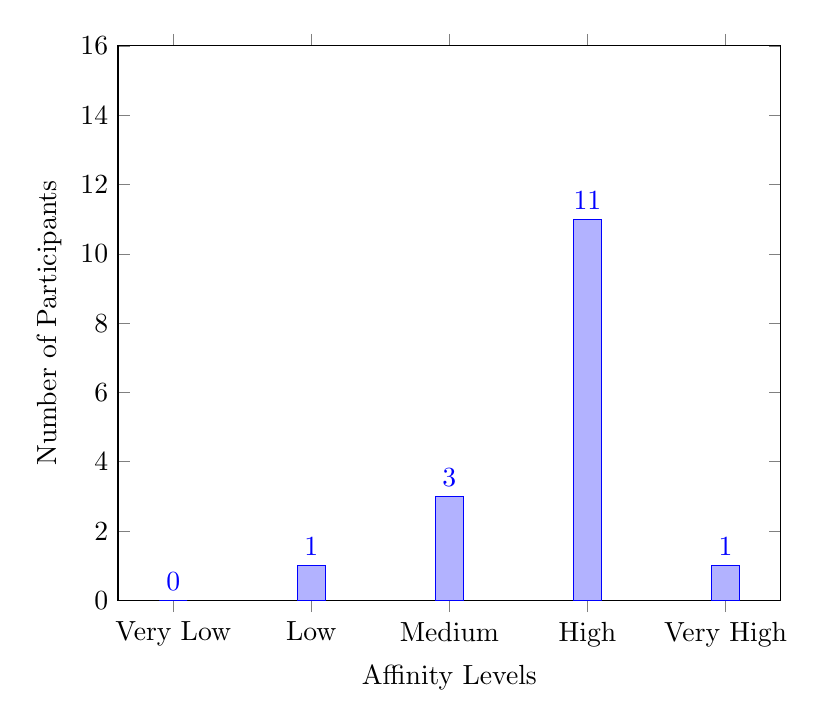
\begin{tikzpicture}
    \begin{axis}[
        ybar,
        symbolic x coords={Very Low, Low, Medium, High, Very High},
        xtick=data,
        nodes near coords,
        nodes near coords align={vertical},
        ymin=0,ymax=16,
        ylabel={Number of Participants},
        xlabel={Affinity Levels},
        %title={ATI-S Scale (Affinity for Technology Interaction)}
    ]
    \addplot coordinates {(Very Low,0) (Low,1) (Medium,3) (High,11) (Very High,1)};
    \end{axis}
\end{tikzpicture}
\caption{Distribution of Affinity for Technology Interaction among participants}
\label{ati}
\end{figure}

A significant aspect of the participant profile is their technological affinity, as indicated by the Affinity for Technology Interaction Short Scale (ATI-S) values. This data revealed a pronounced tendency towards technology, with 12 participants scoring high or very high in technology affinity. This implies that the majority of participants were not only familiar with but also comfortable using technology, which is a crucial consideration in the context of phishing awareness and the effectiveness of warnings.

We opted to use the short version of the ATI scale due to its ability to efficiently measure technological affinity without imposing extensive questionnaire fatigue on participants. The shorter scale offers a balance between comprehensive assessment and participant convenience, ensuring accurate capture of data while maintaining high engagement levels. This is particularly important in studies where the focus is on interaction with technology and where participant time and attention are limited.

\section{Interview Results}

\textbf{Design Response}

Clarity and Legibility: Participants generally found the color red effective in drawing attention, with one noting \textit{"Red is just very catchy"} (P9), highlighting the visual impact of vibrant colors. The legibility of warnings was often a concern, as evidenced by comments such as \textit{"It’s the white on red what makes it difficult to read at times."} (P9), indicating difficulties with text contrast. %Building on this feedback adjustments were made later in the study, starting from particpant 12, such as using a deeper shade of red and a clearer font, aiming to enhance clarity. Doing so did improve participants' response regarding the legibility of the warnings.
    
Impact of Animations: Animations were noted for their effective attention-grabbing capabilities. For instance, one participant mentioned, \textit{"When the text field moves in like this, your eyes automatically move there."} (P1), showing how animations guide viewers' focus. A participant remarked on the possible negative impact of frequent animations, stating, \textit{"Moving warnings are more noticeable than ones that just appear on the screen. But if you put moving warnings on all phishing mails, it might be overwhelming and tire the eyes and mind. A balance is necessary. Maybe being too flashy, could even lead to desensitization over time."} (P5) This comment highlights the delicate balance needed in designing effective alerts that capture attention without leading to user fatigue or desensitization. Some participants also noted that the animations were too slow to appear, \textit{"It would be better if the warnings appeared immediately upon opening the email instead of having a delay"} (P5), which could lead to critical oversights. %Building upon this, we decided to remove the delay for the warning to appear, starting from participant 12. 
    
Placement: Participants commonly observed that warnings placed on the side of the email were less noticeable, often residing in their peripheral vision. As one participant expressed, \textit{"I actually found this one a bit inconspicuous because you have the email body here and the warning there. It reminds me of those advertisements on websites placed on the side of the page."} (P1) Conversely, warnings integrated directly into the email body proved to be more conspicuous. Participants reported that these warnings grabbed their attention immediately upon opening the email, as they were in the direct line of sight while reading the email content. 


\textbf{Perceived Helpfulness}

Context-Aware Warnings (Tooltip on Hover Over Link): This type of warning was generally seen as highly effective because it actively prevents clicks on potentially malicious links. A participant mentioned, \textit{"I believe the one covering the link was the most effective because it immediately prevented interaction."} (P6).
    
Content-Specific Warnings (Signature and Greeting Warnings): This type of warning was appreciated for its specificity, noting that these kind of details are easily overlooked in phishing emails: \textit{"I really liked the signature warnings. That could be something that might not catch the user’s attention at all."} (P5). A common point of criticism was, that this kind of warning is often not applicable, as not every email, especially in a non-business context, ends with a signature or uses a consistent greeting.
      
Generic Banners: This type of warning received mixed feedback due to their positioning and the lack of detailed information they provided. Participants noted its visibility issues and expressed a preference for warnings that include explanatory details about the alert: \textit{"Those that just flew in and had standard text might be the weakest."} (P6). 

\textbf{Preferred Level of Detail}

The "Preferred Level of Detail" code captures participants' responses to different levels of detail in phishing warnings. A key theme that emerged from the interviews was a clear division in preference for either more detailed warnings or simpler alerts. \par
Participants who favored more details appreciated the additional context and explanations provided in the warnings, which helped them understand why an email was flagged as suspicious. One participant stated, \textit{"I preferred the longer ones, because it teaches me how to recognize future phishing attempts."} (P11), emphasizing the educational aspect. Another point mentioned was the fact that a longer explanation might make it easier and more helpful for non tech-savy people. The Greeting Warning with interactive buttons presented a unique challenge during the study. While intended to enhance user engagement by providing direct context and proof, many participants either did not realize the buttons were clickable or hesitated to use them. This hesitation stemmed from a fear that interacting with the buttons might inadvertently lead them into a phishing trap. One participant expressed, \textit{"I wouldn’t like to click on those buttons if I would get such a warning. I don’t really know if I can trust it."} (P16). \par
Conversely, some participants preferred simple warnings, valuing the straightforwardness and immediacy of the message without additional information. This preference indicates that for some users, efficiency and speed in email processing are prioritized over detailed educational content. \newpage

\textbf{Novelties for Participants}

The qualitative data analysis underscored that many participants found the greeting and signature-specific warnings to be novel features. These aspects of the phishing warnings introduced new elements that participants had not previously encountered or considered significant in identifying phishing emails. As one participant reflected, \textit{"I have not seen such tailored warnings in phishing emails, which recognize a specific pattern and tell you why it's a phishing attempt. That is very new to me."} (P13).

\subsection{Refining Warning Design: Incorporating Feedback}
As outlined in section \ref{adjust}, modifications were made to the phishing warning designs beginning with participant 12. 
These changes were positively received, as indicated by subsequent participant feedback. Post-adjustment, there were no further complaints regarding the readability of the text or the timing of the animations, except for a single comment about the red tone being potentially too strong. Participants appreciated the quicker responsiveness and greater clarity of the warnings, which effectively addressed the initial concerns raised about legibility and the timing of animation effects.

%Participants pointed out the necessity for clearer visual cues, leading to a transition to a deeper shade of red to enhance visibility (hex: \#f00c0c). The font choice was also critical; based on suggestions for improved legibility, we shifted to a font that offered greater clarity and readability. More specifically we switched to the font face "Open Sans" and started using more bold fonts. Additionally, the timing and behavior of animations were refined. We observed a common sentiment that immediate, rather than delayed, warning animations were prefered. Therefore, we altered the warning displays to appear instantly as the email was accessed, eliminating any previous delay. A detailed before and after comparision of each warning design is attached in appendix \ref{sec:warnings}.

\section{Eyetracking Results}
\label{sec:eyetrackingres}
The strategic placement of phishing warnings in email interfaces can significantly influence their effectiveness. To investigate the underlying gaze patterns users exhibit when scanning email content and how these can inform optimal warning placement, we established several hypotheses and employed eye-tracking technology for validation. \newline
During the data analysis phase, it was noted that the eye-tracking data for one participant (P13) was significantly lower in sample size compared to others. This anomaly could be attributed to improper seating position or a flawed calibration process. To maintain the integrity and reliability of the analysis, this participant's data was excluded, resulting in a total of 15 eye-tracking samples being considered for the final evaluation.

A full export of our raw eyetracking data is provided the GitHub repository linked in appendix \ref{sec:github}.


\subsection{Hypothesis 1 (H1): Delayed Animation's Influence on Reading Pattern}
We hypothesized that the delayed slide-in animation of warnings would disrupt users' typical email reading pattern. Our eye-tracking data aimed to capture any resultant changes in attention flow, such as an initial focus on the email body shifting to the warning once it appears. \par
\textit{Analysis:} Eye-tracking data indicated no significant disruption in reading patterns due to delayed animations in phishing warnings. Observing the gaze patterns showed that the onset timing of animations, whether immediate or delayed, did not alter the attention flow significantly. Users exhibited similar engagement with immediate and delayed warning presentations, suggesting a uniform approach to processing these visual cues.

\subsection{Hypothesis 2 (H2): Visibility of Side-Placed Warnings} 
Our second hypothesis posited that side-placed warnings would be noticed later in the email reading process—if at all—compared to those placed within the body or at the top. This hypothesis is rooted in the premise that users give precedence to the central content of the email, potentially overlooking peripheral information, which could be confirmed by delayed or absent gaze points on these areas. \par
\textit{Analysis:} The eye-tracking analysis showed that warnings positioned on the side of the email interface consistently captured attention quickly but later than those integrated within the main content. The focus of gaze primarily remained on the central areas of the emails, with peripheral warnings drawing attention only after the central content had been reviewed. This observation was consistent across the study's participants, supporting the hypothesis that side-placed warnings are less immediately noticeable. \newline Detailed eye-tracking metrics reinforce this finding, indicating that it took a median time of \textasciitilde2 seconds for participants to direct their gaze towards side-placed warnings. Notably there were significant outliers where the time to first fixation extended well beyond the median, reaching up 14.01 seconds. These outliers indicate that under certain conditions, the delay in noticing side-placed warnings can be substantially longer.

\begin{figure}[H]
\centering
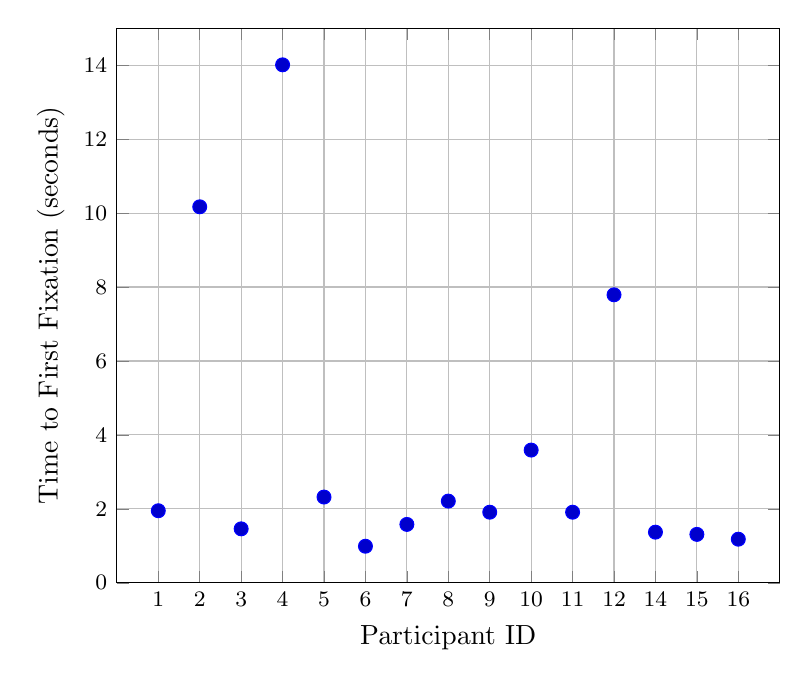
\begin{tikzpicture}
\begin{axis}[
    xlabel={Participant ID},
    ylabel={Time to First Fixation (seconds)},
    grid=major,
    xmin=0, xmax=16, 
    ymin=0, ymax=15,  
    xtick={1,2,...,15}, 
    xticklabels={1,2,...,12,14,15,16}, 
    xticklabel style={font=\footnotesize, rotate=0}, 
    yticklabel style={font=\footnotesize}
]
\addplot+[
    only marks,
    mark=*,
    mark size=2.5pt,
    scatter=false, 
    color=blue, 
    fill=blue  
] table [row sep=\\,y=data, x=seq] {
    seq  data\\
    1    1.95\\ 2    10.17\\ 3    1.46\\ 4    14.01\\ 5    2.32\\
    6    0.99\\ 7    1.58\\ 8    2.21\\ 9    1.91\\ 10   3.59\\
    11   1.91\\ 12   7.79\\ 13   1.37\\ 14   1.31\\ 15   1.18\\
};
\end{axis}
\end{tikzpicture}
\caption{Scatter Plot of Time to First Fixation for Side AOI}
\end{figure}

\subsection{Hypothesis 3 (H3): Prompt Recognition and Sustained Engagement of Body-Integrated Warnings}
Lastly, we theorized that warnings seamlessly integrated directly into the email body (e.g. Greeting or Signature Warning) would not only be detected more swiftly by users but also hold their attention for longer periods. This hypothesis rests on the belief that users are more attuned to and thus more likely to quickly notice and continue to engage with content that is presented within the primary focus of their attention.

\textit{Analysis:} 
Data strongly supported the hypothesis that warnings integrated directly into the email body were detected more quickly and engaged with more thoroughly by users than those placed at the side. The heatmap in figure \ref{fig:heatmap} showed a predominant focus on the central part of the email where these warnings were located. This resulted in not only quicker detection but also significantly longer engagement times compared to warnings placed at the sides of the email. \newline
The analysis of average fixation durations (figure \ref{avgfix}) corroborates these findings, revealing that engagement times for the center AOI were generally longer across participants. However, there were notable exceptions for participants 7 and 14, where the fixation duration on the center AOI was shorter compared to the other participants. 

%This deviation might suggest variability in user interaction with the email content, potentially influenced by individual differences in reading habits or the visual salience of the warnings for these particular participants.
%The extended engagement with the center AOI highlights its effectiveness in not only attracting but also maintaining user attention. This is critical in ensuring that warnings are not only noticed but are also sufficiently processed by users, which is essential for the effective communication of security-related information. 
%The findings suggest that integrating warnings directly within the main content of an email can significantly enhance their noticeability and the extent to which they engage users. Designers might consider positioning crucial information and alerts within the central visual field to maximize their impact. Additionally, understanding the reasons behind the shorter fixation times for specific participants could further refine the design approach, ensuring that warnings are effective across a diverse user base.
%These findings suggest that integrating critical warnings directly into the body of the email is effective in capturing and maintaining user attention. The extended engagement times indicate that users are not only noticing these warnings more quickly but are also spending more time processing the information presented, which is crucial for the effectiveness of such security measures. This extended engagement is corroborated by participant feedback, which highlighted that centrally-located warnings were perceived as more relevant and informative, leading to deeper cognitive processing.

\begin{figure}[H]
\centering
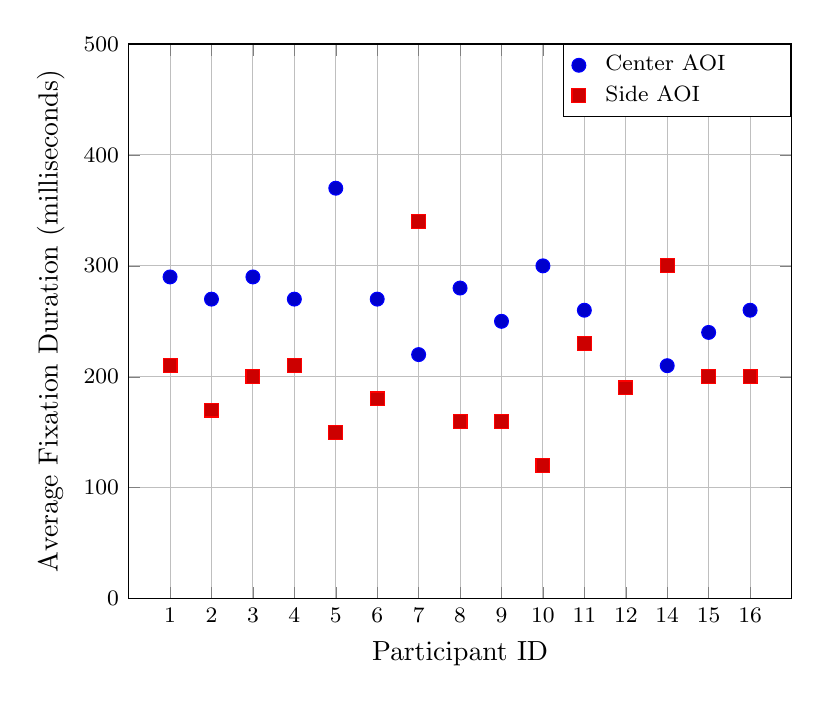
\begin{tikzpicture}
\begin{axis}[
    xlabel={Participant ID},
    ylabel={Average Fixation Duration (milliseconds)},
    grid=major,
    xmin=0, xmax=16, 
    ymin=0, ymax=500,
    xtick={1,2,...,15}, 
    xticklabels={1,2,...,12,14,15,16}, 
    ytick={0, 100,200,300,400,500}, 
    xticklabel style={font=\footnotesize}, 
    yticklabel style={font=\footnotesize},
    legend style={
        at={(1,1)},
        anchor=north east,
        text width=2cm, 
        minimum width=2.5cm, 
        font=\footnotesize 
    }
]
\addplot+[
    scatter,
    only marks,
    mark=*,
    mark size=2.5pt,
    scatter=false,
    color=blue, 
    fill=blue 
] coordinates {
    (1,290) (2,270) (3,290) (4,270) (5,370)
    (6,270) (7,220) (8,280) (9,250) (10,300)
    (11,260) (12,470) (13,210) (14,240) (15,260)
};
\addplot+[
    scatter,
    only marks,
    mark=square*,
    mark size=2.5pt,
    scatter=false,
    color=red, 
    fill=red
] coordinates {
    (1,210) (2,170) (3,200) (4,210) (5,150)
    (6,180) (7,340) (8,160) (9,160) (10,120)
    (11,230) (12,190) (13,300) (14,200) (15,200)
};
\legend{Center AOI,Side AOI}
\end{axis}
\end{tikzpicture}
\caption{Scatter Plot Comparing Average Fixation Duration for Center and Side AOI}
\label{avgfix}
\end{figure}

\begin{figure} [ht]
    \centering
    \includegraphics[width=1\linewidth]{figures/heatmap_overlay.png}
    \caption{Accumulated eyetracking heatmap generated in Tobii Pro Lab}
    \label{fig:heatmap}
\end{figure}

\chapter{Discussion}
\section{Qualitative Feedback}
\subsection{Emerging Themes and Best Practices}
The qualitative feedback analysis illuminates several emerging themes that contribute to the effectiveness of phishing warnings. Reflecting on these, we can delineate best practices for designing phishing warning systems that align with user expectations.

\textbf{Attention-Grabbing without being Overwhelming}

A recurring theme is the delicate balance between capturing users’ attention and avoiding sensory overload. Warnings that are too subtle may go unnoticed, while those that are too aggressive could be dismissed as annoyances. Best practices suggest employing moderate animations and placing warnings within the users' immediate visual field. For example, one participant noted, \textit{"When the text field moves in like this, your eyes automatically move there."} (P2) indicating the value of animated cues. However, animations should not be excessively flashy or complex, as they risk desensitizing users over time. Supporting this, a study on the effects of animation in online contexts found that while animations increase visibility and engagement, they must be balanced to avoid overshadowing important content or overwhelming the viewer \cite{cheung}.

\textbf{Clarity and Contextual Information}

Clarity in warning messages is essential. Participants expressed a preference for warnings with a clear and legible typography set against a contrasting background, improving readability. The use of the color red was frequently mentioned as effective due to its association with caution and urgency. \newline 
Moreover, providing contextual information within the warning, such as the reason an email was flagged and highlighting subtle language cues, such as the greeting, can enhance users’ understanding and prompt more informed action. As one user aptly put it, \textit{"I preferred the longer ones, because it teaches me how to recognize phishing attempts."} (P11), highlighting the educative function. \newline
This emphasis on context-rich warnings aligns with findings from other studies \cite{buono, aneke}, which also highlight the importance of explanatory warnings in phishing emails, thus not only alerting users to immediate threats but also equipping them with knowledge that could prevent future phishing attacks. Such strategies are crucial for improving user understanding and ensuring that warnings lead to informed actions, thereby enhancing the overall effectiveness of phishing defense mechanisms.

\textbf{Trust and Interactivity}

The trustworthiness of warnings is paramount; users must feel confident interacting with them. This includes a hesitance to engage with clickable elements within the warnings due to fear of exacerbating a potential threat. Best practices would, therefore, involve clearly distinguishing warning elements from potential phishing mechanisms and ensuring that interactive components, when used, are immediately recognizable as safe and official parts of the email client interface.

\textbf{Incorporating User Feedback for Iterative Improvement}

The inclusion of user feedback into the design process is not only beneficial but essential for the development of effective phishing warnings. Adjustments made in response to participant insights, such as enhancing color contrast to improve legibility, exemplify how iterative design based on user experience can significantly amplify the effectiveness of security measures. As highlighted in the article by Grobler et al. \cite{grobler} actively engaging users in refining security solutions helps tailor these systems to better meet their needs and expectations, thereby increasing their efficacy and user adoption rates. Best practices would, therefore, advocate for continuous user testing and refinement, ensuring that warnings adapt over time to align with evolving user behaviors and phishing tactics. This proactive approach ensures that security measures remain robust, user-friendly, and effective in real-world scenarios.

\subsection{RQ1: Users’ Perceptions of Phishing Warnings and Their Effectiveness}
To address RQ1 regarding user perceptions and the effectiveness of various phishing warnings in email interfaces, we analyzed qualitative feedback from participants. The effectiveness was assessed based on the ability of warnings to enhance user awareness, encourage appropriate actions to mitigate risks, such as not clicking on malicious links, and improve recognition of phishing threats in future encounters.

\textbf{Perceived Helpfulness and Effectiveness of Warning Types}
\begin{enumerate}
    \item \textbf{Context-Aware Warnings (Tooltip on Hover Over Link):}
    Participants found context-aware warnings extremely effective. These warnings prevent direct interaction with malicious links, thereby immediately mitigating risk. This direct intervention makes them highly valuable in protecting users in real-time.
    \item \textbf{Content-Specific Warnings (Signature and Greeting Warnings):}
    These warnings are appreciated for their specificity and relevance, particularly in environments where consistency is expected, such as professional emails. They provide clear and relevant context by highlighting anomalies in expected email patterns, offering a direct comparison with typical content. Their educational value is significant as they enhance users' ability to identify subtle signs of phishing attempts, which might otherwise be overlooked.
    \item \textbf{Generic Banners:}
    Generic banners received the least favorable feedback. Their effectiveness was often questioned due to poor placement and lack of detailed information, which led to them being easily ignored. Participants compared their noticeability to peripheral advertisements on websites, which are often disregarded due to desensitization. This feedback highlights the importance of not only the placement of warning banners but also the inclusion of specific reasons why an email might be flagged as potentially dangerous, enhancing user understanding and response to phishing threats.
\end{enumerate}

\textbf{Preferred Warning Design}

From the feedback, it's clear that users prefer warnings that are not only visible but also informative. Warnings that blend seamlessly into the user's workflow in the email interface, such as those integrated within the primary content, are particularly effective. These warnings grab attention quickly, provide essential information, and are directly interacted with, enhancing both immediate and long-term phishing threat recognition.


%In examining how users perceive and react to different phishing warning designs, our study revealed clear preferences and perceptions. Users generally found context-specific warnings—those that tied directly to elements like hyperlinks or unusual email signatures and greetings—more helpful and trustworthy. These warnings, by providing clear, relevant context or direct comparisons with typical content, helped users feel better equipped to identify and avoid phishing attempts.

%Conversely, generic banners were often deemed less effective unless they concisely communicated the risks involved. The most effective warnings were those educated users on the reasons behind the warnings and thus enhancing their ability to recognize and respond to phishing threats in future encounters.

%Overall, this feedback underscores the need for phishing warnings that not only capture attention but also educate users, thereby fostering a deeper understanding and stronger defensive actions against phishing attacks.


\newpage
\section{Interpretation of Eye-Tracking Results}
\subsection{Hypothesis Evaluations}

\textbf{Impact of Delayed Animations}

The hypothesis (H1) that delayed animations would disrupt the typical email reading pattern and draw more attention was not supported by the data. The implications suggest that while animations serve as useful attention-grabbing tools, their effectiveness does not necessarily benefit from a delayed presentation. Aligning with the qualitative interview results, it appears that ensuring the visibility of warnings immediately upon email viewing is more crucial for capturing attention and facilitating prompt user reactions.

\textbf{Effective Warning Placement}

The data strongly supported the hypothesis (H3) that warnings integrated into the central viewing area of the email content are noticed more quickly and interacted with more extensively. This result highlights the advantage of aligning warning placements with natural reading behaviors and user expectations, suggesting that integrating security cues directly within the primary content of emails may significantly enhance the detection and responsiveness to phishing attempts. \newline
In contrast (H2), warnings positioned on the periphery of the email interface, such as the sides, were consistently noticed later. Although our data only indicates a slight delay, this brief period can be critical during a hectic workday for instance. Users, under pressure or multitasking, might not immediately spot these peripheral warnings. This oversight offers a window during which they could inadvertently click on deceptive links or interact with other malicious content. \newline
Interestingly, qualitative interviews highlighted a gap between the objective eye-tracking results and participants' subjective experiences. Many participants reported not noticing the side-placed warnings at all. This suggests that while eye-tracking data confirmed visual detection, the warnings were not consciously acknowledged by users, likely due to an automatic filtering process.\newline
Furthermore the presence of outliers where the time to first fixation was exceedingly long underscores the potential severity of this issue. These extreme cases reveal that for some users, the side-placed warnings are not just delayed but might be nearly invisible, akin to the way advertisements on web pages are often ignored due to desensitization. This analogy, supported by the comments of two participants (P1, P9), strengthens the argument that peripheral warnings may be less effective due to a learned tendency to disregard non-central elements, potentially reducing their effectiveness in crucial security contexts.

%\textbf{Hypothesis 1: Delayed Animation's Influence on Reading Pattern:}
%The analysis of eye-tracking data demonstrated that delayed animations did not significantly disrupt or enhance the reading patterns of participants. This finding contradicts our initial assumption that a delayed presentation would shift user focus towards the warnings. The implications suggest that while animations serve as useful attention-grabbing tools, their effectiveness does not necessarily benefit from a delayed presentation. It appears that ensuring the visibility of warnings immediately upon email viewing is more crucial for capturing attention and facilitating prompt user reactions. %This adjustment aligns with user preferences for immediate cues, reinforcing the necessity for warnings to be both conspicuous and timely to effectively counteract phishing threats.

%\textbf{Hypothesis 2: Visibility of Side-Placed Warnings:}
%Eye-tracking data demonstrated that warnings placed on the sides of the email interface were noticed later. This observation aligns with the hypothesis that centrally placed warnings capture attention more effectively.\newline
%Interestingly, qualitative interviews revealed a discrepancy between the objective eye-tracking results and participants' subjective experiences. Many participants reported not noticing the side-placed warnings at all. This suggests that while eye-tracking data confirmed visual detection, the warnings were not consciously acknowledged by users, indicating an automatic filtering process. \newline
%Furthermore, two participants likened the side-placed warnings to advertisements typically found on web pages, which are often ignored due to desensitization. This analogy supports the notion that peripheral warnings may be less effective due to a learned tendency to disregard non-central elements, which could further diminish their impact in critical security contexts.

%\textbf{Hypothesis 3: Prompt Recognition of Body-Integrated Warnings:}
%Eye-tracking data robustly supported the hypothesis that body-integrated warnings are detected more swiftly and engaged with more thoroughly. The centralized focus of users on the email body naturally led to quicker and more intense interactions with warnings placed in this area. This result highlights the advantage of aligning warning placements with natural reading behaviors and user expectations, suggesting that integrating security cues directly within the primary content of emails may significantly enhance the detection and responsiveness to phishing attempts.

\subsection{RQ2: Gaze Patterns and Warning Placement}
\textbf{Central Gaze Concentration} 

The analysis of common gaze patterns among users when scanning email content has revealed key insights into the strategic placement of phishing warnings. The eye-tracking data from our study indicate a strong tendency for users to focus their initial attention on the center of the email content, which aligns with natural reading behaviors. Thus, warnings that were integrated directly into this central area were noticed more swiftly and engaged with more thoroughly compared to warnings placed at the periphery. 

\textbf{Implications for Warning Placement} 

The findings underscore the necessity of placing phishing warnings within the primary visual path to ensure they are both seen and acted upon promptly. This strategic placement leverages natural gaze behaviors to enhance the visibility and effectiveness of warnings. Furthermore, these insights suggest that the design of email interfaces should consider how information is visually prioritized by users, utilizing this knowledge to design more effective phishing defense mechanisms.

\section{Limitations}

\subsection{Participant Diversity and Sample Size}
The majority of our participants were drawn from a similar demographic group, predominantly consisting of university students and young adults within the same age range and academic environment. Moreover, a significant portion of participants demonstrated a high Affinity for Technological Interaction (ATI), as illustrated in figure \ref{ati}. This heightened technological comfort and skill among our sample may not accurately represent the broader population's varying levels of technological proficiency. The lack of diversity in our sample, both demographically and in terms of technological affinity, could limit the generalizability of our findings across a broader population and potentially introduce biases in the evaluation of our phishing warnings. For example, older adults might interpret and respond to visual cues differently due to variations in technological fluency and cognitive processing speeds, which may differ markedly from the responses observed in younger, more technologically adept participants \cite{age}. \newline
Additionally, the iterative design adjustment made based on participant feedback later in the study highlighted another significant limitation related to sample size. After implementing changes to the warning designs, it was planned to test these modifications with eight additional participants. Unfortunately, only four additional participants were able to participate in the study. This smaller-than-expected sample size of participants might not provide a sufficiently robust dataset to draw definitive conclusions about the effectiveness of the redesigned warnings.

%\textbf{Recommendations for Future Research}
%Given these factors, future research should strive to include a more diverse participant pool and ensure an adequate sample size to enhance the robustness and applicability of the findings. Expanding the demographic range to include varied ages, professions, and educational levels would provide a more comprehensive understanding of how different user groups perceive and react to phishing warnings, thereby supporting the development of more universally effective measures. Additionally, employing larger sample sizes in testing phases can help to ensure that findings are statistically significant and reflective of a wider user base.

\subsection{Study Setup and Ecological Validity}
The use of a controlled lab environment to conduct this study poses significant limitations regarding ecological validity. Participants were aware that their actions were being observed, potentially influencing their behavior—a phenomenon known as the Hawthorne effect \cite{jim}. This awareness can alter natural responses and may not accurately reflect their behavior in less controlled environments. \newline
Furthermore, the artificial nature of the study environment can significantly impact participants' risk perception \cite{garfinkel}. Since the risk to personal data is non-existent in a simulated phishing attack, participants' reactions to warnings and their decision-making processes might not truly reflect their actions in a real threat scenario. This discrepancy can skew results related to actual risk perceptions and behaviors, potentially leading to overestimations of the effectiveness of warning systems in genuine contexts.

%\textbf{Recommendations for Future Work}
%To enhance the ecological validity and real-world applicability of future phishing studies, it is advisable to extend the study design to include actual user environments. This expansion could involve the development and integration of a phishing detection algorithm tailored for real-world application. Such an adaptation would allow the testing of our phishing warnings within live settings, moving beyond the constraints of simulated environments used in our current methodology. Integrating these systems in real user scenarios would not only yield more authentic data but also provide a robust assessment of the effectiveness of phishing warnings and user responses under normal usage conditions. This approach promises a more accurate evaluation of the practical impact and reliability of anti-phishing strategies in everyday digital interactions.

\chapter{Conclusion}
\label{sec:conclusion}
This thesis has extensively investigated the impact of various visual warning designs on user responses to phishing threats in email clients. The use of eye-tracking technology and qualitative feedback has provided a deep understanding of how different warning strategies affect user behaviour and engagement.

The research conclusively demonstrates that integrating warnings directly within the email content markedly enhances both the immediacy of user reactions and their overall engagement with the warnings. These findings underline the importance of prominent, context-rich warnings that are easily visible and provide actionable information to users.

Furthermore, the study highlights the crucial role of educational content in warnings. Clear, informative warnings not only alert users to immediate threats but also educate them, enhancing their ability to identify similar threats independently in the future. This dual function of warnings is vital in the ongoing battle against phishing, as well-informed users are the first line of defense in cybersecurity.

However, the study also highlights significant opportunities for expansion in both scope and realism for future research. A crucial first step is broadening the participant pool to include a more diverse range of ages, professions, and educational backgrounds, and increasing sample sizes to ensure findings are robust and generalizable. This will enhance our understanding of how different user groups perceive and react to phishing threats, supporting the development of more universally effective defensive measures. Additionally, to significantly boost ecological validity, future studies could integrate phishing detection research into real-world user environments. This advancement might entail the development and application of phishing detection algorithms capable of operating effectively within users' naturalistic settings. Such a move would not only provide more authentic data but also allow for a robust assessment of phishing warning effectiveness under typical usage conditions.

Looking forward, the rapid advancement of artificial intelligence and large language models opens new frontiers for phishing defense. These technologies could be leveraged to develop more adaptive, personalized phishing detection and prevention strategies, enhancing the precision and responsiveness of warnings. For instance, AI could analyze user behavior to tailor warnings to individual risk profiles or detect subtle phishing attempts that evade traditional detection methods. This proactive and technologically innovative approach is crucial in an era where cyber threats are continually evolving, thus ensuring the digital safety of users globally. As cybercriminals become more sophisticated, integrating cutting-edge technologies into cybersecurity measures will be essential for staying ahead of threats and safeguarding digital interactions.




 
\printbibliography

All links were last followed on \today{}.

\appendix
\chapter{Appendix}

\section{GitHub Repository}
\label{sec:github}
This public repository contains everything related to the study (e.g. Plugin Source, E-Mail Samples, Transcripts etc.).\par
\href{https://github.com/yunuseyvz/Bachelorthesis-Phishing-Warning-Techniques}{https://github.com/yunuseyvz/Bachelorthesis-Phishing-Warning-Technique}


\section{Study Protocol}
\label{sec:protocol}
\textbf{Welcome and Consent:}
\begin{itemize}
    \item Introduction to the study.
    \item Participants read and sign the consent form.
    \item Notification of screen, audio recording, and eye-tracking data collection. All data is anonymized.
\end{itemize}

\textbf{Preparation:}
\begin{itemize}
    \item Use a non-rolling chair for better eye-tracking results.
    \item Overview of the eye tracker and setup instructions.
    \item Setup of Mozilla Thunderbird with necessary addons.
    \item Setup of Tobii Pro Lab with a second screen for the moderator.
    \item Calibration of eye tracker integrated into Tobii Pro Lab's timeline.
\end{itemize}

\textbf{Conducting the Study:} Participants are allowed to ask questions throughout if anything is unclear.

\textbf{Part 1: Email Sorting (Approximately 10 Minutes):}
\begin{itemize}
    \item Role-play as an employee at ``Cloudtech'', sorting emails as if it's their actual work inbox. Note: To simplify the process user may only delete or not delete emails. No further actions are needed.
    \item Encourage to think aloud while sorting.
    \item Interaction with emails, including links and attachments, is allowed.
    \item Discussion follows after about 10 minutes.
\end{itemize}

\textbf{Part 2: Detailed Interview (Approximately 10 Minutes):}

Before moving on to the interview participants are debriefed. The warning designs are shown and explained again. See appendix \ref{sec:interview} for the Interview Questions

\textbf{Conclusion of the Session:} Compensation of €10 via PayPal/Transfer or 1 MMI point.


\section{Interview Questions}
\label{sec:interview}
These are the questions posed to the participants in the second phase. Note that the interview was semi-structured so deviations and follow up questions were possible.

\textbf{General Perception:}

\begin{itemize}
    \item How did you generally perceive the warnings? Did they immediately stand out?
    \item Follow-up questions, e.g., if "Good", ask why exactly good or bad.
    \item Were there elements in the warnings that particularly stood out to you? What caught your attention the most?
    \item What role did the warning notices play in your decisions?
\end{itemize}

\textbf{Effectiveness of the Warnings:
}
    \begin{itemize}
        \item How do you assess the effectiveness of the various warning notices presented to you during the study?
        \item Were there any warning notices you found particularly helpful or less helpful?
        \item Each warning notice had 2 versions (simple/detailed). Which version do you prefer, and why? (Show the warnings again)
    \end{itemize}

\textbf{Design of the Warning Notices:}

    \begin{itemize}
        \item How do you evaluate the design of the warning notices (e.g., color, placement, animations)? Did these influence your attention?
        \item How do you assess interactive elements in warning notices (e.g., greeting warning)?
        \item Do you have any suggestions for improving the design of the warning notices?
    \end{itemize}

\textbf{Personal Behavior:
}
    \begin{itemize}
        \item Were there any pieces of information in the warnings that you hadn't paid attention to before?
        \item How do you usually handle emails once there's a suspicion of phishing? Or what specifically do you look at once there's a suspicion?
    \end{itemize}

\textbf{Feedback:
}
    \begin{itemize}
        \item Do you have any suggestions on how we could improve the study in the future?
        \item Do you have any other questions or comments?
    \end{itemize}

\newpage   
\section{Warning Designs}
\label{sec:warnings}
Below is an overview of version 1 of each warning type.

\begin{figure} [H]
\centering
\begin{subfigure}{.5\textwidth}
  \centering
  \includegraphics[width=.8\linewidth]{figures/banner1_old.png}
  \caption{Variant 1}
\end{subfigure}%
\begin{subfigure}{.5\textwidth}
  \centering
  \includegraphics[width=.8\linewidth]{figures/banner2_old.png}
  \caption{Variant 2}
\end{subfigure}
\caption{Generic Banner (Version 1)}
\end{figure}

\begin{figure} [H]
\centering
\begin{subfigure}{.5\textwidth}
  \centering
  \includegraphics[width=.8\linewidth]{figures/hover1_old.png}
  \caption{Variant 1}
\end{subfigure}%
\begin{subfigure}{.5\textwidth}
  \centering
  \includegraphics[width=.8\linewidth]{figures/hover2_old.png}
  \caption{Variant 2}
\end{subfigure}
\caption{Tooltip Warning on Link Hover (Version 1)}
\end{figure}

\begin{figure} [H]
\centering
\begin{subfigure}{.5\textwidth}
  \centering
  \includegraphics[width=.8\linewidth]{figures/sig1_old.png}
  \caption{Variant 1}
\end{subfigure}%
\begin{subfigure}{.5\textwidth}
  \centering
  \includegraphics[width=.8\linewidth]{figures/sig2_old.png}
  \caption{Variant 2}
\end{subfigure}
\caption{Signature-Specific Warning (Version 1)}
\end{figure}

\begin{figure} [H]
\centering
\begin{subfigure}{.5\textwidth}
  \centering
  \includegraphics[width=.8\linewidth]{figures/greeting1_old.png}
  \caption{Variant 1}
\end{subfigure}%
\begin{subfigure}{.5\textwidth}
  \centering
  \includegraphics[width=.8\linewidth]{figures/greeting2_old.png}
  \caption{Variant 2}
\end{subfigure}
\caption{Greeting-Specific Warning (Version 1)}
\end{figure}

\section{QDA Codebook}
\label{sec:qda}
Below is the list of codes developed and utilized during the qualitative data analysis process of our study.
\begin{itemize}
    \item Design Response: This code looks into the overall aesthetic and functional reception of the warning designs by the participants.
    \begin{itemize}
        \item Clarity and Legibility: Evaluates how easily the warnings can be read and understood.
        \item Impact of Animations: Assesses how motion and dynamic elements in the warnings affect user attention and understanding.
        \item Placement: Considers the effectiveness of where warnings are located within the email interface.
        \item Potential Improvements: Gathers participant suggestions on how to enhance the warning designs.
        \item User Attention: Analyzes how conspicuous or inconspicuous these warnings are to the users.
        \begin{itemize}
            \item Conspicuous: Warnings that are immediately noticeable.
            \item  Inconspicuous: Warnings that tend to be overlooked.
        \end{itemize}
    \end{itemize}
    \item Novelties for Participants: Identifies aspects of the phishing warnings that were particularly novel or unexpected to the participants.
    \item Perceived Helpfulness: Explores participants' perception on each warnings helpfulness.
    \begin{itemize}
        \item Negative: Participant feedback that highlights shortcomings or ineffective aspects of the warnings.
        \item Positive: Positive reactions that underscore the effectiveness and utility of the warnings.
        \item Prefered Complexity: Explores participants' preferences for the complexity of the information provided in the warnings.
        \begin{itemize}
            \item More Details: Preference for detailed and informative warnings.
            \item Simplicity: Preference for straightforward, minimal warnings.
        \end{itemize}
    \end{itemize}
\end{itemize}

%\input{latexhints/latexhints-english}

\pagestyle{empty}
\renewcommand*{\chapterpagestyle}{empty}
\Affirmation
\end{document}
